\documentclass[aps,prb,reprint,showpacs,floatfix,superscriptaddress, onecolumn, nofootinbib, 10pt]{revtex4-2}

\usepackage{amsmath,amsthm,amssymb}
\usepackage{graphicx}% Include figure files
\usepackage{dcolumn}% Align table columns on decimal point
\usepackage{bm}% bold math
\usepackage{color}
\usepackage{epsfig}
\usepackage{multirow}
\usepackage{mathrsfs}
\usepackage{hyperref}
\usepackage{cleveref}
\usepackage{epstopdf}
\usepackage{subfigure}
\usepackage{autobreak}
\usepackage{todonotes}
\usepackage{physics}
\usepackage{bbm}
\usepackage[normalem]{ulem}
\usepackage[margin=0.5cm]{geometry}

\usepackage[absolute,overlay]{textpos}

%Macros for mathematical notations

\newcommand{\V}[1]{\boldsymbol{#1}} %# vector
\newcommand{\M}[1]{\boldsymbol{#1}} %# matrix
\newcommand{\Set}[1]{\mathbb{#1}} %# set
\newcommand{\D}[1]{\Delta#1} %# \D{t} for time step size
\renewcommand{\d}[1]{\delta#1} %# \d{t} for small increment
\newcommand{\av}[1]{\left\langle #1\right\rangle } %take average

\newcommand{\sM}[1]{\M{\mathcal{#1}}} %matrix in mathcal font
\newcommand{\dprime}{\prime\prime} % double prime
%\global\long\def\i{\iota}
%\renewcommand{\i}{\iota} %i for imaginary unit
%\renewcommand{\i}{\mathsf i} %i for imaginary unit
\newcommand{\follows}{\quad\Rightarrow\quad} %=>
\newcommand{\eqd}{\overset{d}{=}} %=^d
\newcommand{\spe}[1]{\mathscr{#1}}  %important quantities in mathscr font
\newcommand{\eps}{\epsilon}

\newcommand{\response}[1]{{\color{black}#1}} % for authors' response
\newcommand{\comment}[1]{{\color{blue}#1}} % for referee's comment


\begin{document}
\preprint{Preprint}

\title{Response to Referee Comments for Manuscript NJP-117075}
\author{Mahbub Rahaman, Akitada Sakurai, Analabha Roy}
\date{\today}

\maketitle

\vspace{1em}

\noindent \textbf{Response to the Referee: 2's comment}
\begin{enumerate}
	\item {\bf Major Comments}
	\begin{enumerate}
		\item The referee comments on, \comment{``System size dependence: The manuscript presents insightful results for a system size
				of N=8; however, a crucial aspect remains unexplored – the dependence of the
				findings on the system size. How do the observed dynamics and stability vary with an
				increase in system size?"}\\
		
		\response{
			We thank the referee for this suggestion. We have extended our investigation beyond system size N=8 . The results in figure(9) exhibits melting in DTC phase accompanied by beats at almost all possible spin interactions (defined by $\beta$) and coupling strengths in regional magnetization ($M^z_A$) curves in region A. To understand this melting in DTC observation, we have considered sizes N =4,6,8,10 and numerically calculated $M^z_A$ at and obtained corresponding FFTs for an extended time period upto $8 \times 10^4$T at DTC/DL point.  DTC/DL point is the first root of Bessel function of drive parameters $\frac{4h}{\omega}$. 
			
			We have numerically calculated the beats frequency for each case of $\beta$'s and spin coupling strengths (weak and strong) and plotted in figure(12) in revised manuscript. We observe that the beats frequency for each cases decreases with increase in system size N. This confirms that the stability of the DTC-DMBL chimeralike order increases with increase in N for all selected $\beta$'s and coupling strengths. At thermodynamic limit where $N\rightarrow\infty$, the corresponding beat frequency vanishes manifesting a perfectly stable chimeralike order. We have revised the manuscript describing dependence of findings on the system size in a subsection, titled ``4.3. System size dependent stability in chimeralike order'' in page no.19.
		}
	
		\item The referee comments on, \comment{``Influence of rotational error $\epsilon_B$: The manuscript effectively investigates the
			impact of $\epsilon_A$={0.03,0.05,0.1} on the chimera states, leaving the role of $\epsilon_B$, set to 0.9, less discussed. How does varying $\epsilon_B$ impact the chimera
			states?"}\\
		
		\response{We thank the referee for pointing out the issue. We have considered additional rotation error $\epsilon_B = 0.6\; \&\; 0.8$ maintaining a constant value of $\epsilon_A = 0.03$. We have considered drive parameters at CDT/DL point and numerically calculated local magnetization $\expval{\hat{S}^z}$ for all $\beta$'s and spin coupling strengths in figure(7) in revised manuscript. We found that the DTC-DMBL order lacks stability at each cases. The stability of DMBL phase in region B decreases with increase in $\epsilon_B$. This does have direct proportional dominance over the stability of DTC phase in region A. Additionally we observed that the local magnetization in region A varies equally for all-to-all interaction, but for shorter ranges $\expval{\hat{S}^z}$ decays rapidly with decrease in spin interaction ranges ($\beta >0$) as well as with increase in relative distance from jounction between the regions A $\&$ B. We have added this discussion in detail in section(3) page no.12 and from line no. 238 to the end of the section.
			
		In order to get a general comprehension over the stability of DTC-DMBL chimeralike order, we extended our investigations for a large set of $\epsilon_A$ and $\epsilon_B$ and calculated regional magnetization $M^z_A$ and $M^z_B$ at CDT/DL point for selected $\beta$'s and coupling strengths. We have plotted the obtained $M^z_{A,B}$ values in figure(8) in page no.15. We observe that $\epsilon_A$ and $\epsilon_B$ are the key element to control over the stability and selection of DTC and DMBL phases in regions. At extreme opposite condition when $\epsilon_A \sim 0$ and $\epsilon_B\sim1.0$ the DTC-DMBL chimera is most stable. When $\epsilon_B$ is considered for smaller values (<0.9) maintaining a constant $\epsilon_A = 0.03$, we observe that both of the region gains melting DTC phase with gradual decrease in $\epsilon_B$ (see panels-a,b,c,d). We have investigated also for the cases when $\epsilon_A\sim\epsilon_B$ which are found not to exhibit the DTC-DMBL chimeralike order. Interestingly, when we consider a fixed $\epsilon_B=0.1$ and increase $\epsilon_A$ we observe DMBL in region A and DTC in region B at extreme opposite case when $\epsilon_A=0.1$ and $\epsilon_B=0.9$. We have included this discussion in the revised manuscript in section '4.1. Regional Magnetization' on page 14 from line number 294 to 336.
		
		}
		\item The referee comments on, \comment{``\underline{Higher root of Bessel function and stability of chimera states:}"}\\
		\begin{enumerate}
			\item \comment{``The paper introduces a higher root of the Bessel function without explicitly justifying its significance. The importance of this higher root and its relevance to the stability
				of chimera states need clarification. How does the selection of a higher root impact the system's behavior, and why is it crucial for the observed dynamics?"}\\
			
			\response{We thank the referee to point out the mistake. To obtain DMBL in $T_2$ cycle, the drive parameters should be considered in a manner that the ratio $\frac{4h}{\omega}$ is one of the roots of Bessel function $\mathcal{J}_0\left(\frac{4h}{\omega}\right)$ which is denoted as `CDT/DL point' as discussed in Appendix-A. There is no restriction on selection over the root of the Bessel function regarding CDT/DL point. We have corrected this issue by defining `CDT/DL point' corresponding to the first root of $\mathcal{J}_0\left(\frac{4h}{\omega}\right)$ at page no,\ref{Put the page number line number etc.} and maintained it through out in the manuscript and updated all the figures in revised manuscript with no change in results with comparison to the earlier manuscript. 
			}\\
			\item \comment{``Moreover, the statement “The stability of the chimera order diminishes even if there is a minor deviation from the CDT/DL point” (page 15, lines 43-44) implies that chimera states might not be stable under slight deviations from the CDT/DL point. This raises a critical question regarding the practical implementation of creating chimera states in experiments. To address this, it would be valuable for the paper to explore potential techniques or strategies aimed at stabilizing the DMBL part of the chain. Elaborating on practical considerations and potential solutions would enhance the paper's applicability and contribute to a more comprehensive understanding of the proposed model."}\\
			
			\response{We thank the referee for the comment. We have considered the drive parameter ratio $\frac{4h}{\omega}$ at fixed to CDT/DL point (which we have chosen to be the first root of the Bessel function for our numerical simulations) which is 2.4048 and the point away from CDT/DL we considered to be 6.0 which is $\sim0.40$ value differ from its closest Bessel function root ($\mathcal{J}_4 =6.3802$). At this point DMBL as well as chimeralike state is unstable. This deviation $~0.40$ is a major deviation from any CDT/DL point. So our claim on instability of chimeralike order at minor deviation in earlier manuscript was incorrect. The minor deviation should be smaller than this regarding the scale of drive parameter ratio. 
				
			To investigate the stability of chimeralike order around the CDT/DL point we have introduced a minor deviation($\Delta_h$) in range between $\in[-0.05, 0.05]$ to the drive amplitude (h) which corresponds to the CDT/DL point at constant drive frequency $\omega = 20$. We also considered the spins are all up polarized initially and system size to be N=8 and $\beta=0$. One can consider otherwise $\beta$'s; however that would necessitate larger system size which spans larger matrices in product space. We numerically evolve the system for a few time cycles upto 20T and calculate the fidelity ($F_n = \abs{\braket{\psi(0)}{\psi (20T)}}^2$) which measures the closeness of the initial state  to the state of the system at 20T. We have plotted $F_n$ for different $\frac{4\Delta_h}{\omega}$ in figure below. The minor deviation region is filled with gray color. 
			\begin{figure}[h!]
				\begin{center}
					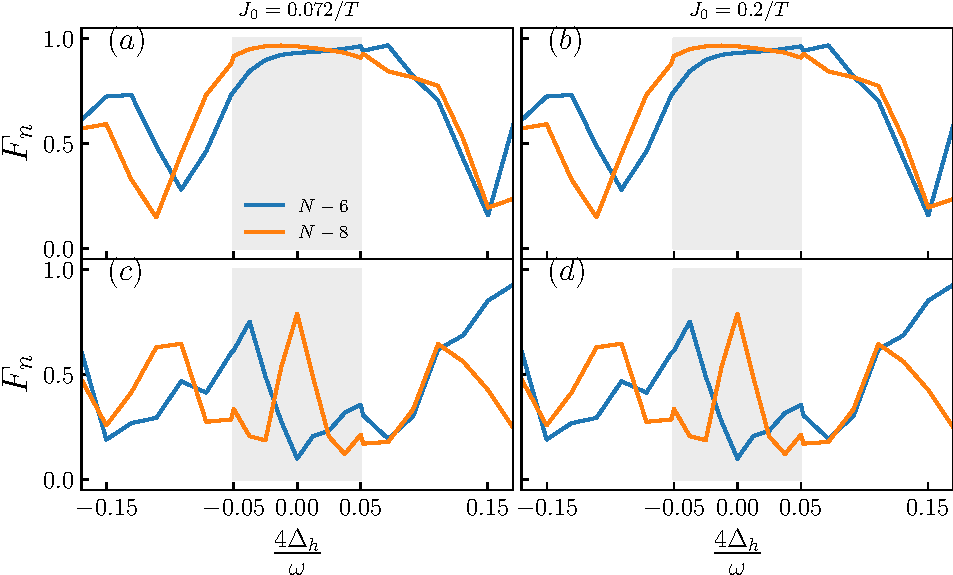
\includegraphics[width=10cm]{./figs/figure14.pdf}
				\end{center}
				\caption{Fidelity is plotted against several deviation values $\frac{4\Delta_h}{\omega}$ for different system size (N). The CDT/DL point is denoted by gray dashed line where $\frac{4\Delta_h}{\omega}=0$. Weak (a-panel) and strong (b-panel) is considered. The fidelity is found to be enough large around CDT/DL point (gray-colored region).}
				\label{Fig:aroundCDT}
			\end{figure}
			We found that $F_n$ is sufficiently large ($>0.85$) around the CDT/DL point for both of the spin coupling strengths. We have revised the manuscript at section 4.4 by replacing the sentence ``...even if there is a minor devation..." with ``... at significant deviation..." at page no.20,line no. 403. Additionally we have discussed this issue at Appendix-C at page no.28. 
			}
		\end{enumerate}
	
		\item The referee comments on, \comment{``\underline{DTC phase stability and entanglement entropy:}"}
		\begin{enumerate}
			\item \comment{``The paper seems to be intended for an audience from DTC and MBL/DMBL fields. However, for broader accessibility and comprehension, a brief introductory paragraph about realization and fundamental aspects of DTC within DMBL
			systems would be beneficial. How is DTC defined in these systems, and what are its fundamental properties? Additionally, how is $\omega$ chosen in relation to the periodicity of the Hamiltonian? Moreover, a preliminary explanation of how analyzing the time evolution of local magnetization and its FFT contributes to defining DTC would greatly enhance reader comprehension."}\\
		
			\response{
			}
			\item \comment{``It is important to clarify the results shown in Fig. 7, where the behavior of regional magnetization might confuse new readers in the DTC field. This figure suggests that regional magnetization decreases over time under strong coupling and all-to-all interactions, which at the first glance seems to contradict the main text’s assertion that these conditions correspond to stable chimera states. Therefore, a comment  explaining how the magnetization relates to FFT based on the results would be helpful for correctly understanding the results."}
			\item \comment{``There appears to be inconsistency in the analysis of EE and regional magnetisation along with FFT. EE is shown for almost two times longer dynamics that regional magnetization and FFT. Could the authors provide a comparison of regional  magnetization and its FFT for the extended time frames considered for entanglement entropy?"}
		\end{enumerate}
		\item The referee comments on, \comment{``\underline{Applications of chimera state:} The introduction of Section 4 briefly touches upon applications of chimera states, but it lacks depth. How can the chimera state findings be applied in practice? Expanding on potential applications and providing references to existing literature will be beneficial. This would enrich the discussion and highlight the practical relevance of their findings."}
	\end{enumerate}

	\item[] {\bf Minor Comments}
	\begin{enumerate}
		\item The referee says, \comment{``\underline{Page 6, lines 30-31 and page 18, lines 47-48:} please add a reference to the Baker-Campbell-Hausdorff formula, e.g. [67] as in the Appendix B, page 22, lines 44-45"}\\
		\item The referee says, \comment{``\underline{Page 6, lines 46-48:} clarify what is $\mathcal{J}_0$, e.g. “of the higher roots of zeroth-order Bessel function $\mathcal{J}_0$”"}\\
		\item The referee comments on, \comment{``\underline{Page 8, caption of Fig. 3:}"}
		\begin{enumerate}
			\item The referee says, \comment{``refine the caption for clarity: “plotted for different values of amplitude h of the periodic drive. The x-coordinate plots 4h/$\omega$, where drive frequency is kept constant $\omega$=20..."}\\
			\item The referee says, \comment{``The first such point is shown...” $\rightarrow$ “The first two points are shown..."}
		\end{enumerate}
		\item The referee comments on, \comment{``\underline{Page 9, caption of Fig. 4:}"}
		\begin{enumerate}
			\item The referee says, \comment{``This is the suggestion of a notation change for smoother reading: “Site(i)” → “i”, 
			e.g. “for each i-th spin at region A (i=0,1,2,3) and region B (i=4,5,6,7)...”. To implement this modification consistently: change the x-coordinate labels in the Fig. 4 from “Site(i)” → “i”, and update accordingly the main text/ figures/ captions to
			maintain consistency"}\\
			\item The referee says, \comment{``Revise “spin coupling ($J_0$=0.027/T)” $\rightarrow$ “spin coupling ($J_0$=0.072/T)”"}
			\item The referee says, \comment{``Please add also the information for which root of the Bessel function the plot is obtained."}
		\end{enumerate}
		\item The referee comments on, \comment{``\underline{Page 10, Fig. 5:}"}
		\begin{enumerate}
			\item The referee says, \comment{``Define $M_A^z$, which appears in the y-label, in the main text or the caption for
				clarity. The formal introduction of regional magnetization occurs in Section 4, while
				Fig. 5 is situated within Section 3."}\\
			\item The referee says, \comment{``Specify a CDT/DL point, i.e. to which root of the Bessel function it corresponds"}
		\end{enumerate}
		\item The referee comments on, \comment{``\underline{Page 11, lines 50-51:} Specify “a CDT/DL point...” while throughout the paper the root of the Bessel function is changing, e.g. Fig. 4 and Fig. 5"}
		\item The referee comments on, \comment{``\underline{Page 13, Fig 8:} Correct the notation “$\omega/\omega_D$” → “$\Omega/\omega$”"}
		\item The referee says, \comment{``Ensure all paper captions are reviewed for consistency. Additionally, include all relevant
			parameters in the captions that would enable interested readers to reproduce your
			results effectively."}
	\end{enumerate}

	\newpage
	\noindent \textbf{Response to the Referee: 3's comment}
	\begin{enumerate}
		\item The referee says, \comment{``My main concern is regarding the context in which the word “chimera” has been used
			in this work. The word chimera was originally used for the co-existence of synchronized and unsynchronized dynamics of coupled “identical” oscillators in the “Phys. Rev. Lett. 93, 174102 (2004)” which was initially discovered in the following
			works “Y. Kuramoto and D. Battogtokh, Nonlinear Phenom. Complex Syst. 5, 380 (2002), S. I. Shima and Y. Kuramoto, Phys. Rev. E 69, 036213 (2004)”. The surprise that led to the discovery of the chimera state resided in the fact that all the
			subsystems were identical and were subjected to the same environment but behaved differently only due to different initial configurations. But in this and the earlier work mentioned by authors “Phys. Rev. Lett. 126, 120606 (2021)”, regions A and B are under different drive conditions. Hence, the spins in these regions are not under identical environments. In such a configuration, it is trivial that both regions can behave differently since they are subjected to different drive conditions. Hence, this co-existence of different phases under inhomogeneous drive conditions for different
			regions does not fall under the novel phenomenon of “chimera”.\\
			
			I understand that this issue arises due to the fact that the related work “Phys. Rev. Lett. 126, 120606 (2021)” has referred to this phenomenon as a “chimera state”, even though one of the authors from the same paper has used the definition of the identical oscillator in their earlier work “Phys. Rev. E 92, 062924 (2015)”. Therefore, I request the authors either remove the word chimera completely or use the word “chimeralike state” which has been used in the work “Phys. Rev. E 103, 012214 (2021)” where authors have discovered a chimeralike state in almost-identical oscillators. Along with this, authors should provide a clear distinction that the definition of “chimeralike state” used in this work differs from the definition involving identical oscillators and follows from the earlier work “Phys. Rev. Lett. 126, 120606 (2021)” and “Phys. Rev. E 103, 012214” which involve non-identical systems. I
			suppose this is crucial to avoid misunderstandings and further confusion about the novel “Chimera State” for the readers of this reputed journal."}\\
		
		\item The referee says, \comment{``Adding to the previous point on chimera-like states, it would be interesting to see if
			the chimera state emerges even for almost the same drive conditions for regions A
			and B, i.e. for $\epsilon A \approx \epsilon B$ where they only differ by a small value."}\\
		\item The referee says, \comment{``Authors can also investigate the onset of the chimera state as a function of $\epsilon A$ - $\epsilon B$."}\\
		\item The referee says, \comment{``To avoid confusion, the 45th line of Page 2 should be modified to indicate that the concept of “time crystal” was introduced by Frank Wilczek, not just the Discrete time crystals."}\\
		\item The referee says, \comment{``$J_0$ is not defined after equation 7 in the main text."}\\
		\item The referee says, \comment{``Recent works have not been included in the manuscript, I list some of the recent work on chimera states in time crystals and observation of discrete-time crystals for the consideration of authors:."}
		\begin{enumerate}
			\item \comment{``Observation of a Dissipative Time Crystal”, Phys. Rev. Lett. 127, 043602 (2021)"}
			\item \comment{``Observation of a Prethermal U(1) Discrete Time Crystal”, Phys. Rev. X 13, 041016 (2023)"}
			\item \comment{``Observation of time crystal comb in a driven-dissipative system”, arXiv:2402.13112 (2024)}
			\item \comment{``Exotic synchronization in continuous time crystals outside the symmetric subspace”, arXiv:2401.00675 (2024)"}
		\end{enumerate}
	\end{enumerate}
\end{enumerate}
		
		

	
	
\noindent \textbf{Summary of important changes to the  manuscript}
\begin{enumerate}
	\item write the changes you have made$\dots$.
\end{enumerate}
\end{document}